This experiment was carried out at the Idaho Accelerator Center (IAC), using their short-pulsed linear accelerator, which is an L--band frequency (1300 MHz) electron linear accelerator.
See section~\ref{beam} for the accelerator parameters used during the experiment.
Figure~\ref{fig:Facility} shows a top-down diagram of the experimental arrangement.

\begin{figure}[h]
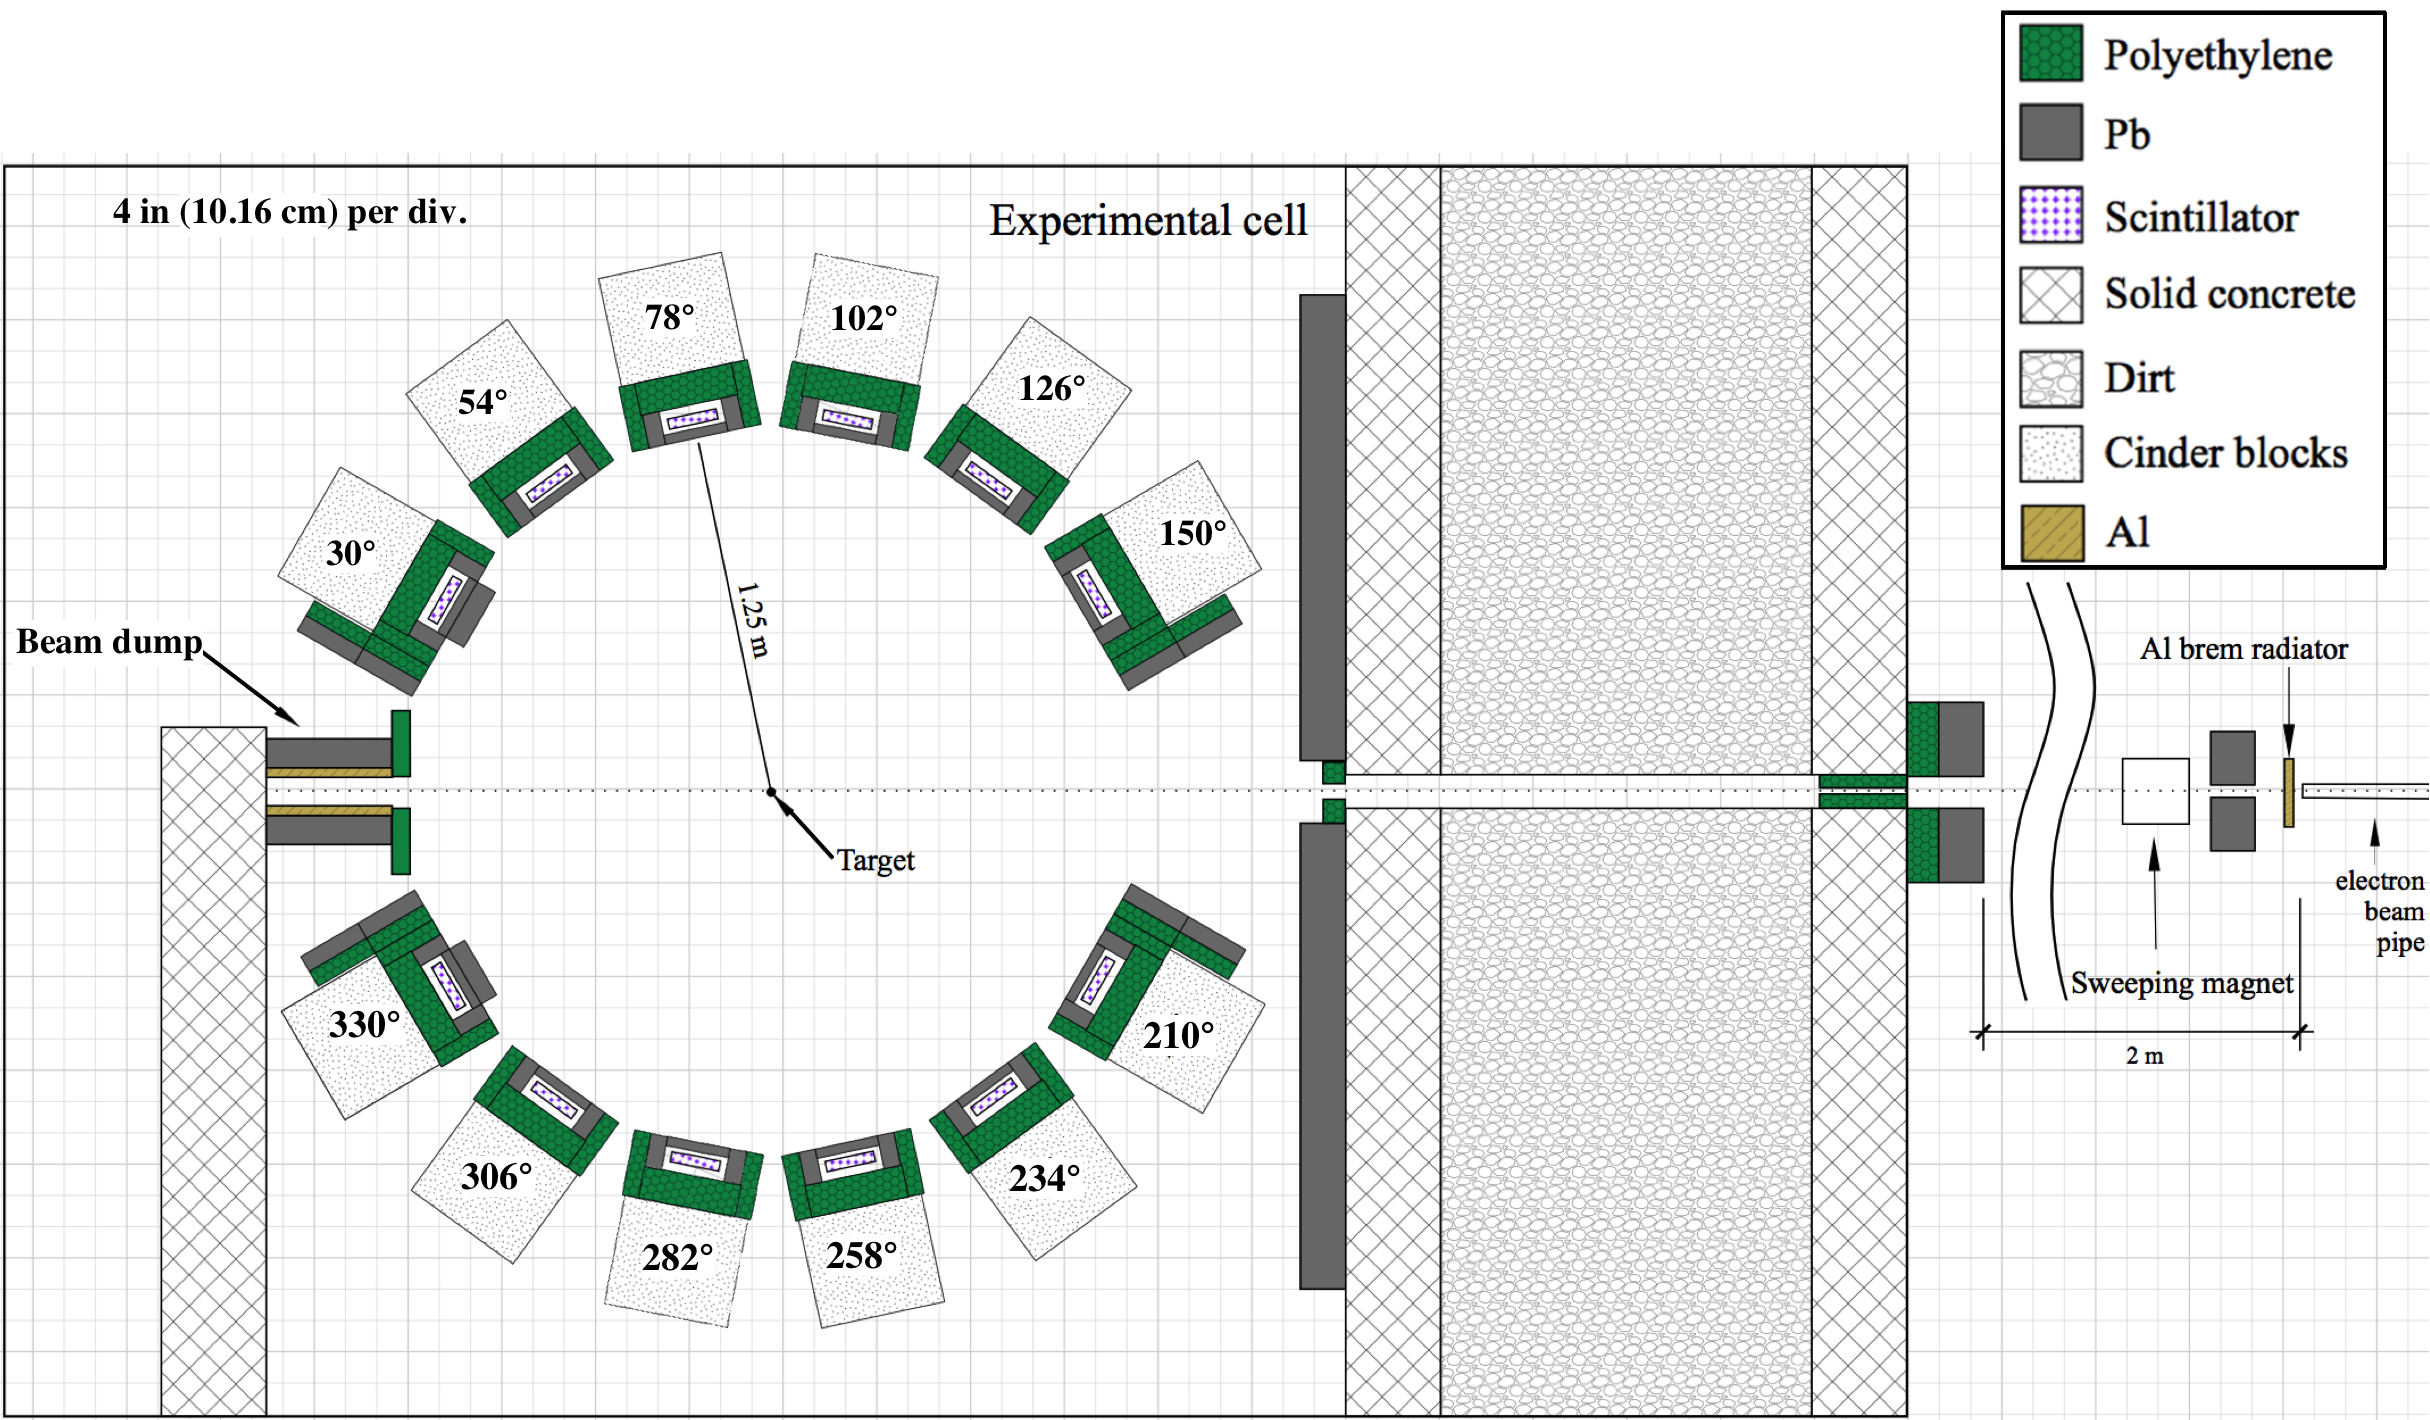
\includegraphics[width=\FigFacilitySize\textwidth, angle=\Angle]{ExpArangment.jpg}
\caption{To-scale, top down diagram of the experimental setup.
An electron beam impinges upon a 3.8 cm thick Al radiator, and the resulting bremsstrahlung beam enters the experimental cell from the top of the figure.
The supporting structure for each detector has been labeled according to the angle, in degrees, between the center of each detector and direction of the incoming photon beam.
The fission target, a 0.05$\times$2$\times$4 cm$^3$ $^{238}$U cuboid, is rotated slowly about the vertical axis in order to replicate the effect of using a cylindrical target.
}
\label{fig:Facility}
\end{figure}
\figFacilityBarrier

\subsection{Detectors}
\label{subsection:detectors}
The detection system measures neutron position and time of flight (ToF), which is defined as the time taken for a particle to travel from the fission target to a detector.
The purpose of the ToF measurement is to determine the kinetic energy of detected neutrons and to distinguish between photons and neutrons.
The detection system's positional precision is $\pm$9~cm, which results in an average opening angular precision of $\pm6^{\circ}$ for a target to detector distance of 1.25 m. 
The detection system consists of fourteen shielded scintillators made from Polyvinyl Toluene (PVT) arranged in a ring around the target (see Figs.~\ref{fig:Facility} and~\ref{fig:DetGeom}).
Attached to both ends of each scintillator are 10-cm long, non-scintillating, ultra-violet transmitting, plastic light-guides.
A Hamamatsu 580-17 photomultiplier (PMT) tube is fixed to each light-guide using optical glue.
In order to increase the chance that scintillation light remains inside the scintillator, the scintillators were polished to remove micro-imperfections and were then wrapped in reflective aluminized mylar.
\begin{figure}[]
    \centering
    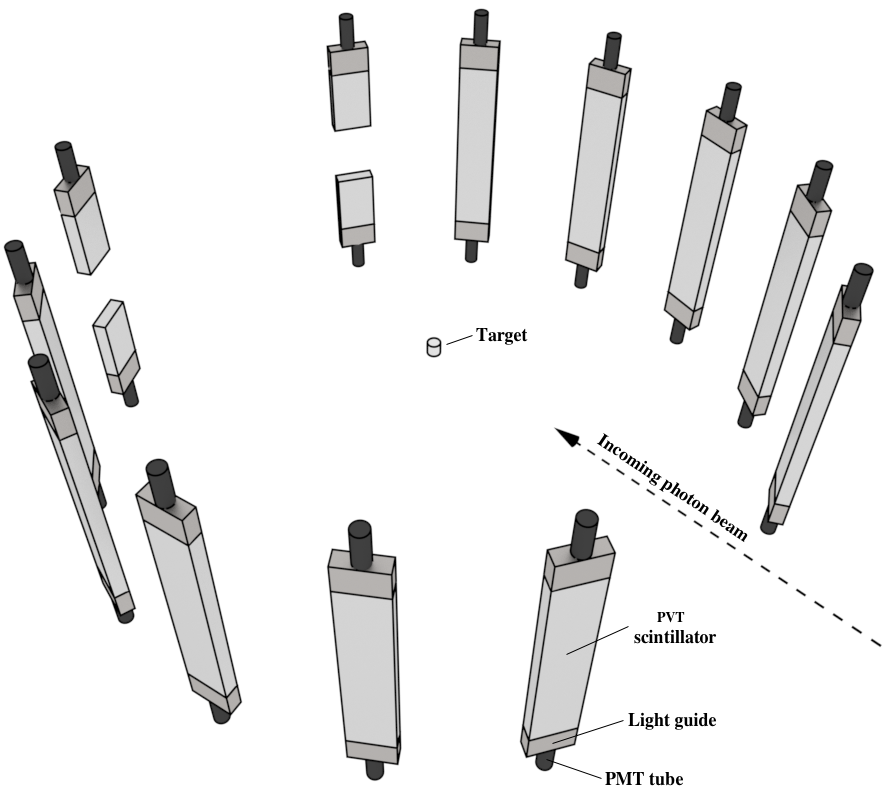
\includegraphics[width = \figsize\textwidth]{Detectors.png}
    \caption{3-D rendering of the bare, unshielded scintillators, along with PMTs and light guides.
    Most of the open space between the scintillators was occupied by shielding, as seen in Fig.~\ref{fig:Facility}.
    }
    \label{fig:DetGeom}
\end{figure}

Ten of the fourteen scintillators had dimensions of 76.2$\times$15.2$\times$3.8 cm$^3$.
The remaining four, located nearest to the beam line at $\pm$ 30$^{\circ}$ with respect to the beam, had dimensions of 25.4$\times$15.2$\times$3.8 cm$^3$.
These scintillators, 1/3 the length of the rest, are the result of the segmentation of two normally sized scintillators in order to lower the relatively high photon detection rates near the beam line.
Prior to segmentation, a photon was registered in the forward-most detectors at a rate of about 0.9 photons per pulse, and because the electronics were operated in single hit mode (see section~\ref{sec:electronics}), this greatly reduced the effective neutron detection efficiency.
After segmentation and optimization of shielding, the photon detection rate was about 0.2 photons per pulse in each segmented detector.\onlyThesis
The segmented detectors also differ from the rest in that they were instrumented with only a single PMT, and therefore provide a comparatively lower precision in energy and position measurements.
In order to test for systematic errors that may have resulted from the use of the segmented detectors, opening angle measurements were compared with and without their use, and the differences were well within experimental errors.

The relative efficiencies of the neutron detectors as a function of neutron energy and detector location were calculated by dividing the measured yields by the yields of neutrons from the SF of $^{252}$Cf according to MCNP.
The results are shown in Fig.~\ref{fig:RelErgEfficiency}.
Note that the effects of the uncertainty in measured neutron energy (seen in Fig.~\ref{fig:ErgUncertainty}) are folded into this calculation.
The analysis techniques described in section~\ref{Analysis} are designed to eliminate the effects of detector efficiency from the final result.
\begin{figure}[]
    \centering
    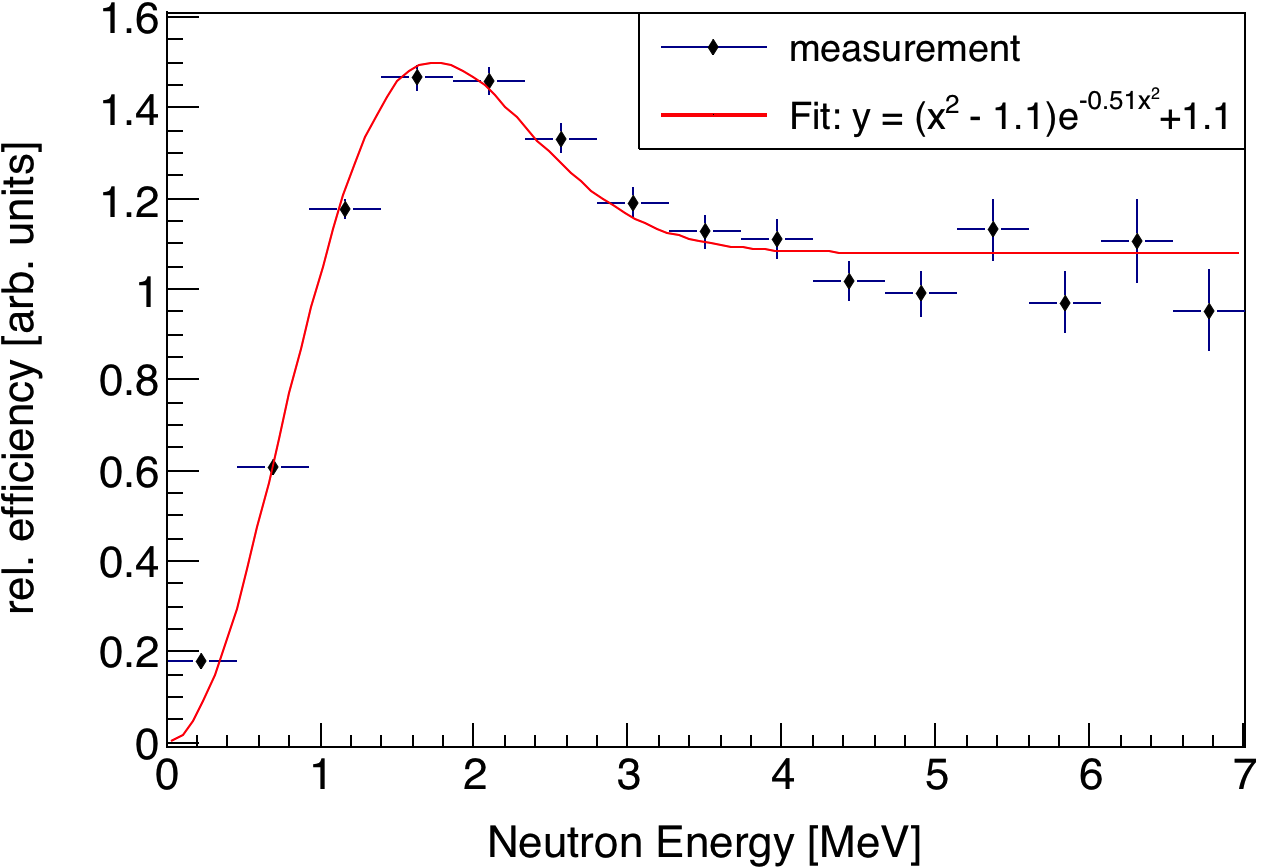
\includegraphics[width = \figsize\textwidth]{RelErgEfficiency.png}
    \vspace{10cm}

     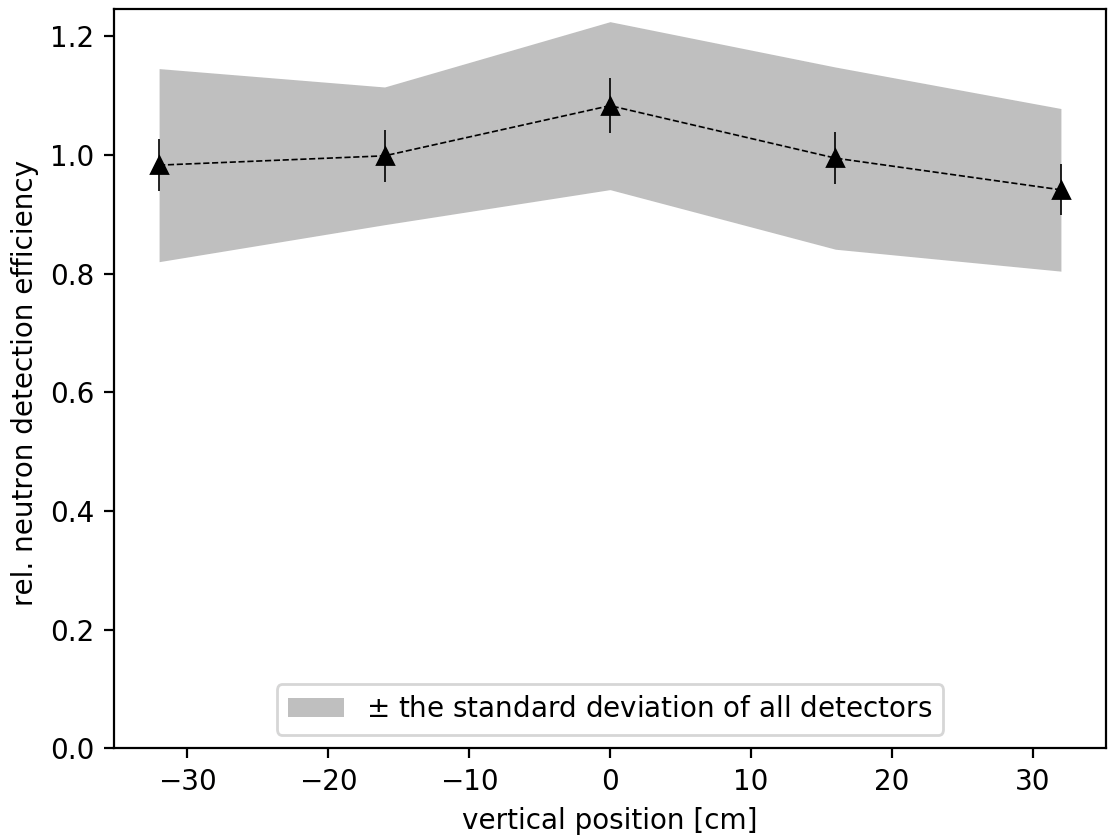
\includegraphics[width = \figsize\textwidth]{RelPosEfficiency.png}
     
       \caption{(top) The mean relative neutron detection efficiency of all detectors as a function of neutron energy is calculated by dividing the measured energy distribution by the known energy distribution of neutrons from the SF of $^{252}$Cf. The relative efficiency differs from detector to detector, as demonstrated by the shaded region, which corresponds to the standard deviation of the relative efficiencies of all detectors. The error bars represent the uncertainty in the mean. (bot) Mean relative neutron detection efficiency as a function of the reconstructed position along the detectors longest axis. }
    \label{fig:RelErgEfficiency}
\end{figure}

\subsection{Detector Shielding}
\label{shielding}
The detector shielding, depicted in Fig.~\ref{fig:shielding}, was constructed using lead and polyethylene with the aim of reducing detector cross-talk, the detection of photons, and noise.
The sides of each scintillator were shielded with 5 cm of lead followed by 5 cm of polyethylene to reduce the chance of neutron cross-talk.
Lead was not placed behind the scintillators after an MCNP-POLIMI simulation indicated that the additional lead would significantly increase cross-talk rates.
Instead, 10~cm of polyethylene was placed behind the scintillators.
For a detailed discussion about the issue of cross-talk, see section~\ref{crosstalk}.

The front face of each detector was subject to the highest photon flux due to the scattering of the bremsstrahlung beam from the target.
The detection of a photon renders the given detector unable to detect any subsequent fission neutrons from the same pulse due to the detector recovery time.
Lead mitigates this problem by reducing photon flux, but has the side effect of scattering neutrons.
If a neutron scatters prior to being detected, the ToF measurement and position reconstruction are corrupted.
The extent of measurement errors caused by lead shielding was quantified using an MCNP simulation, and, accordingly, 2.5~cm of lead was placed along the front face of the detectors.
This diminished photon detection rates to reasonable levels, and, according to the simulation, leads to a root-mean-square error in opening angle and ToF of 1$^{\circ}$ and 0.3~ns, respectively, due to neutron elastic scattering.

Because of the particularly high photon flux at the sides of all detectors located directly adjacent to the beam, an additional 2" of lead was placed along the sides of these detectors.
For the same reason, an additional 2" of lead was also placed along the front faces of the detectors farthest downstream, located at $\pm30^{\circ}$ from the beam line.
The differences in shielding design among the detectors can be seen in Fig.~\ref{fig:Facility}.
\begin{figure}
    \centering
    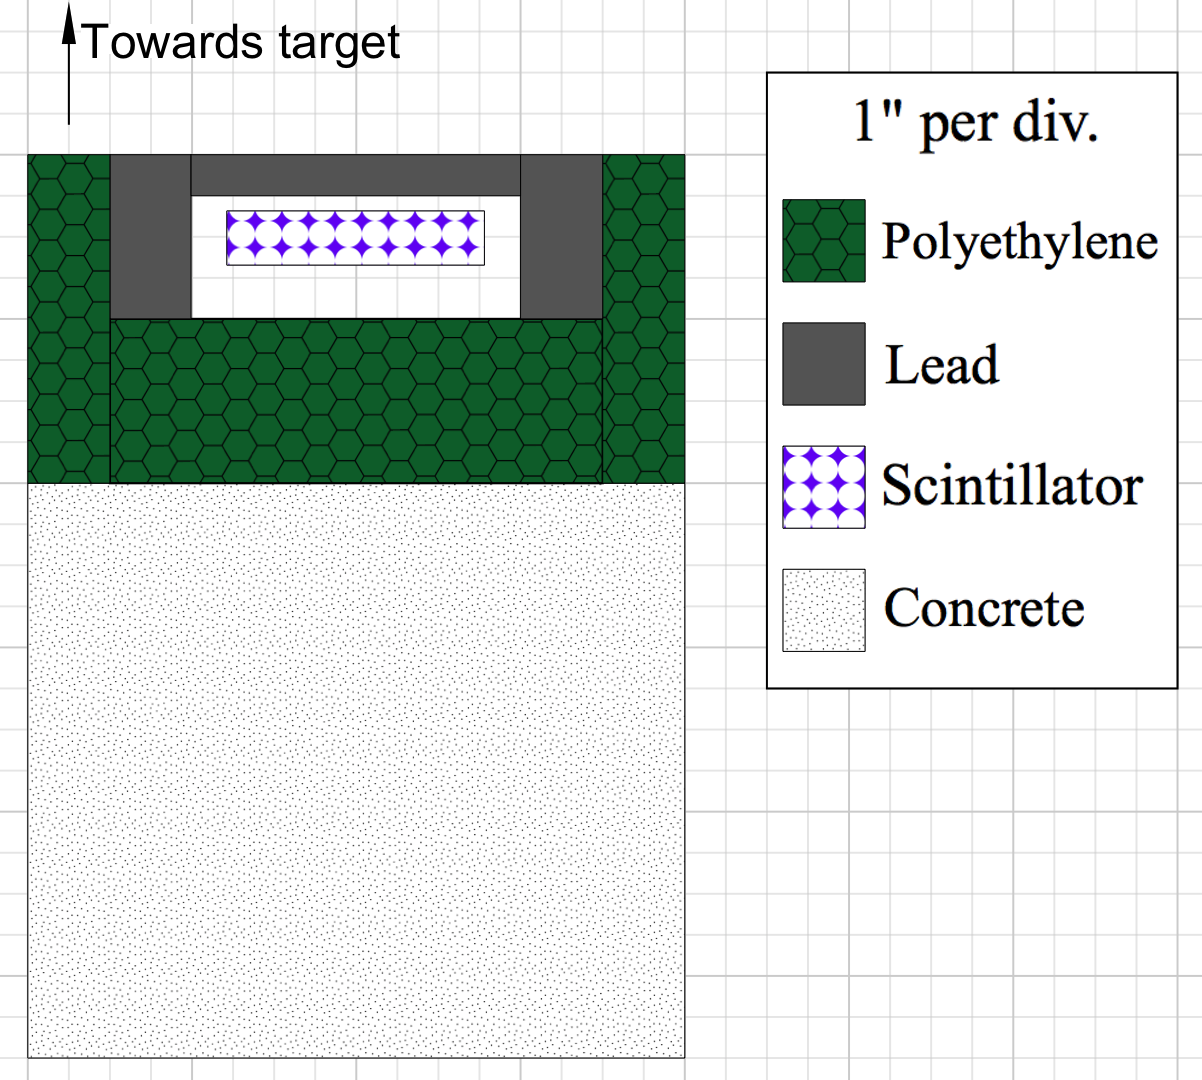
\includegraphics[width = \FigShieldingSize\textwidth]{DetShielding.png}
    \caption{Detector shielding was designed to reduce the detection of photons, room return, and detector cross-talk.}
    \label{fig:shielding}
\end{figure}

\subsection{Bremsstrahlung Photon Beam}
\label{beam}
In order to ensure that all correlated neutrons produced are due to fission, the bremsstrahlung end-point energy was set to 10.5~MeV, safely below the ($\gamma, 2n$) threshold of 11.28~MeV for $^{238}$U.
Aluminum was chosen for the bremsstrahlung radiator because it has a neutron knockout threshold above the energy of the electron beam, which ensured that the radiator would not be a source of fast neutrons with the potential to interfere with the experiment.
A sweeping magnet was placed downstream from the bremsstrahlung radiator to remove charged particles from the photon beam.
Following the sweeping magnet, the beam traveled through a series of polyethylene and lead collimators on its way into the experimental cell in which the target was located (see Fig.~\ref{fig:Facility}).
Figure~\ref{fig:BremDist} shows the energy distribution of photons that reach the target according to an MCNP simulation that modeled the collimation and production of the bremsstrahlung photons.

The electron beam pulse width was set to 3~ns at a repetition rate of 240~Hz with a 1.1~A peak current.
The 3~ns pulse width was small compared to the median neutron ToF of 80~ns, and thus made a small contribution to the uncertainty in the neutron energy determination.
\begin{figure}[h]
\centering
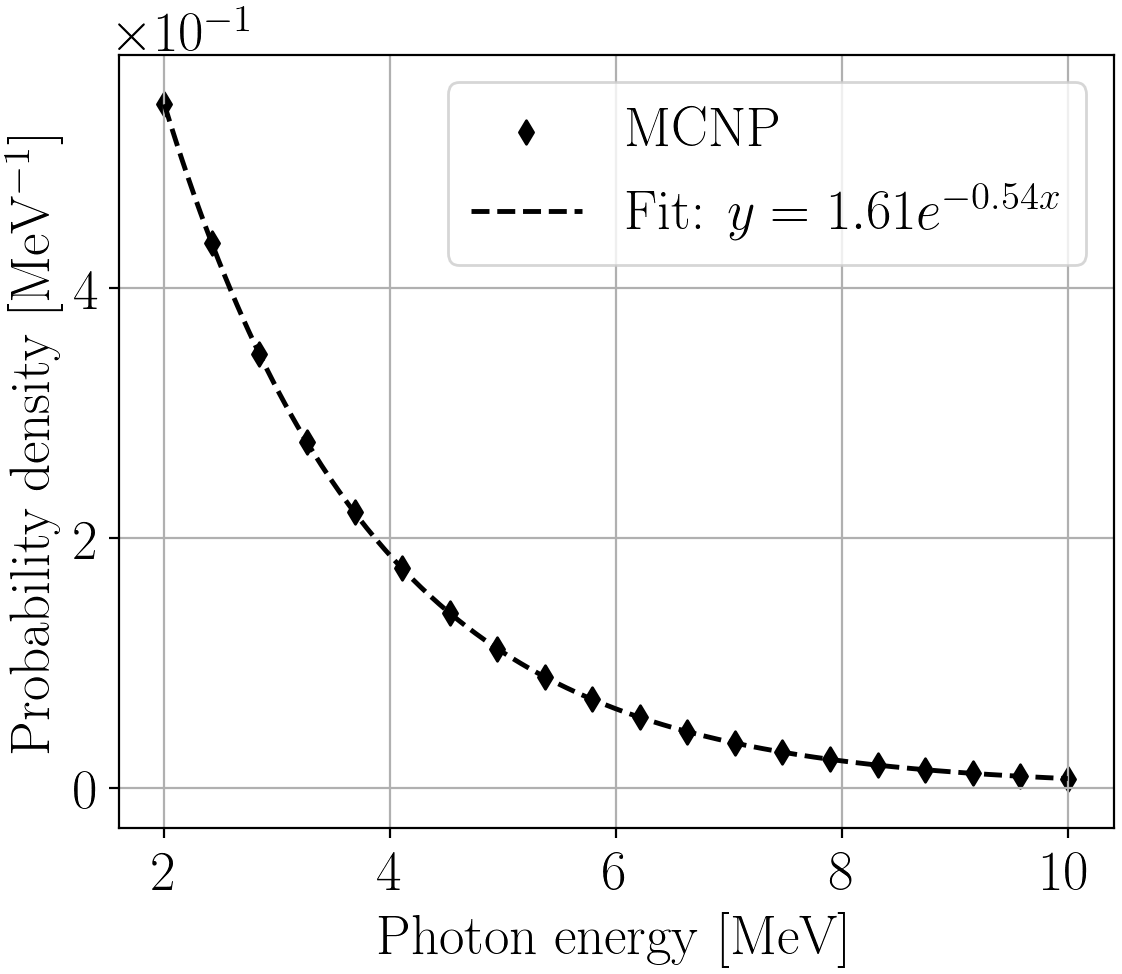
\includegraphics[width=\FigBremDistSize\textwidth]{MCNPBremDistribution.png}
\caption{MCNP simulation of the energy distribution of the bremsstrahlung photons that reach the fission target. Photons with an energy below 2 MeV are excluded.}
\label{fig:BremDist}
\end{figure}

\subsection{DU Target}
\label{subsection:targets}
A depleted uranium (DU) target in the shape of a thin strip with dimensions of 4$\times$2$\times$0.05 $\text{cm}^3$ and a mass of 7.6 g was used as the primary target.
$^{238}$U was chosen as the fission target because it is an even-even nucleus, and as a consequence, the fission fragments are emitted with a high degree of anisotropy with respect to the photon beam direction~\cite{1977FragAss}.

Any target comprised of heavy nuclei has a significant potential to scatter fission neutrons before they exit the target.
This is cause for concern, because neutrons that scatter from heavy nuclei are likely to be deflected at large angles, resulting in the measurement of $\theta_{nn}$'s unconnected to the underlying fission kinematics.
As discussed in detail in section~\ref{subsection:Elastic_scattering}, an MCNP simulation estimated that 6\% of reconstructed $\theta_{nn}$'s are perturbed due to neutron scattering within the $^{238}$U target.
Moreover, it is more likely that neutrons emitted along the wide, 2~cm, axis of the $^{238}$U target undergo a scattering event than neutrons emitted along the thinnest, 0.05~cm, axis.
As a result, detectors located collinear to the widest axis of the target would see relatively fewer neutrons due to increased scattering along this axis. 
This bias is removed by slowly rotating the target about the vertical axis during data acquisition at a rate of one rotation per 8 seconds.
%Because this measurement is of a statistical process, rotating the target gives the same effect as if a cylindrical target were used.
%See section~\ref{subsection:Elastic_scattering} for discussion of issues regarding neutron scattering within the fission target.  

\subsection{Electronics}
\label{sec:electronics}
A data acquisition system based on the NIM/VME standard was used.
A schematic of the data acquisition logic is shown in Figure~\ref{fig:WiringDiagram}.
The PMTs are supplied negative voltages ranging from 1300 to 1500 V by a LeCroy 1458 high voltage mainframe.
Analog signals from the PMTs were fed into a leading edge discriminator (CAEN Mod. N841) with input thresholds ranging from 30 mV to 50 mV.
The threshold and supply voltages were determined individually for each detector to minimize noise, while simultaneously matching the efficiencies of all the detectors as closely as possible.
Logic signals from the discriminator were converted to ECL logic and fed into a CAEN model V1290A TDC.
The timing of signals from the PMTs were always measured relative to a signal from the accelerator provided at the beginning of each pulse.
Even though a multi-hit TDC was used, only the first signal in each pulse from any given PMT was taken into account due to concerns over dead-time within the electronics and signal reflections within the cables.
On the software side, the CODA 2.5 ~\cite{CODA} software package developed by Jefferson Laboratory was used to read out the data from the TDC and digitally store it for analysis.

\onecolumngrid
\begin{figure}[h]
\centering
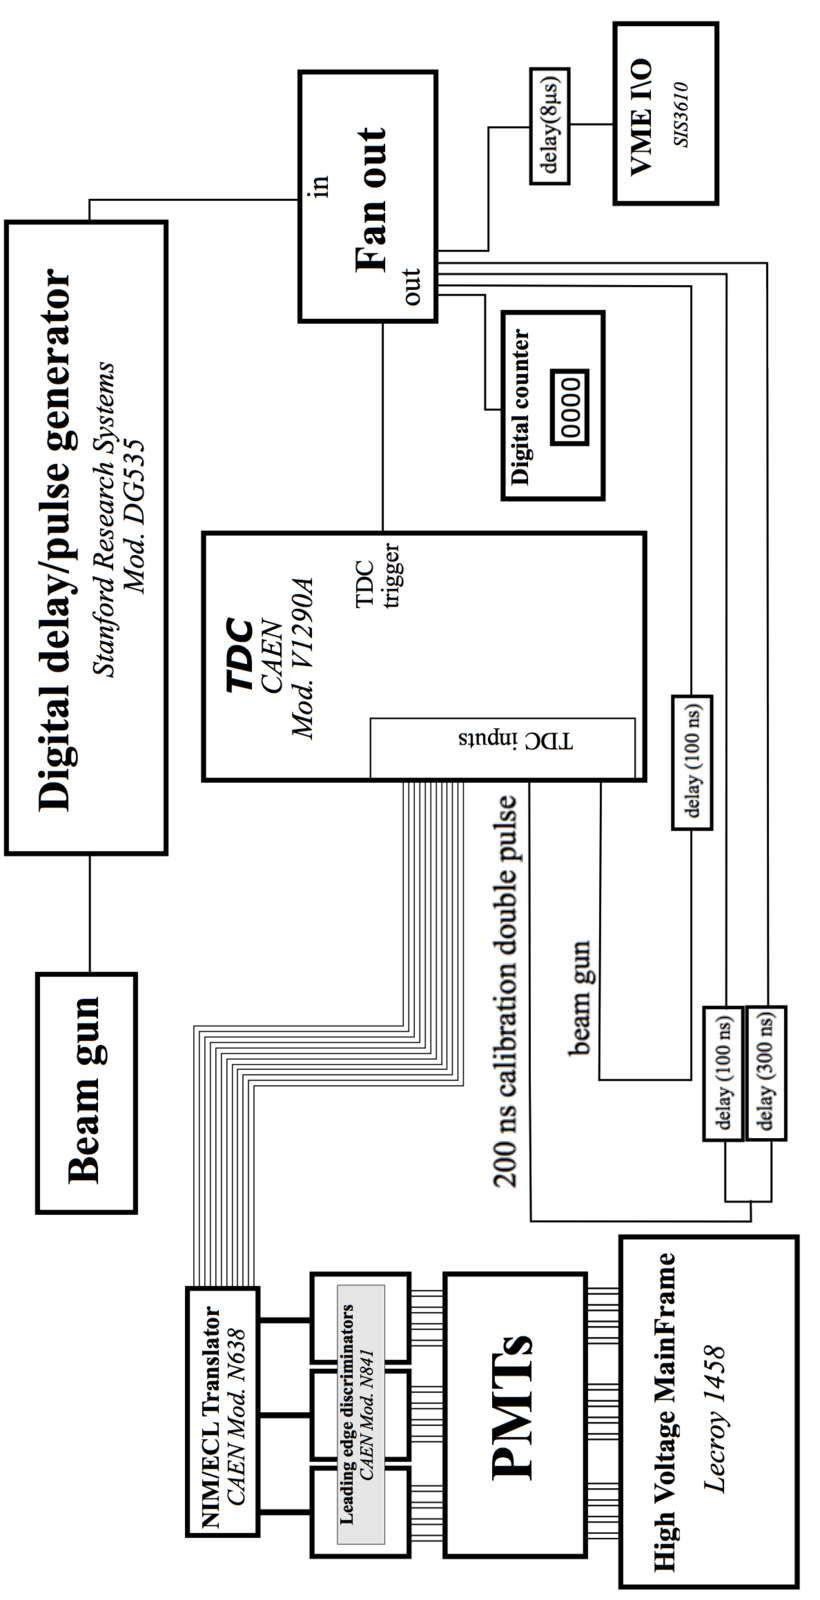
\includegraphics[width=\textwidth, angle=\WireAngle]{WiringDiagram.png}
\caption{Wiring diagram of the electronics setup. }
\label{fig:WiringDiagram}
\end{figure}
\figWiringDiagramBarrier
\twocolumngrid

